% 19.11.2025; 12:11:06


\section{Einführung Softwaredesign}%
\begin{frame}%
    \frametitle{Softwaredesign -- Einführung}

    \begin{table}[H]
        \begin{tabularx}{\linewidth}{|lX|}
            %         &\\
            % Software&Das Programm das geschrieben wird\\
                    &\\
            Software-Design&
                Das Planen von Software um bestimmte Ziele zu erfüllen\\
                           &\\
            Design Patterns\footnote{""Entwurfsmuster""}&Standard Lösungen für Probleme bei der Softwareentwicklung \\
                                                        &Werden entdeckt, \underline{nicht} erfunden\\
                    &\\
                    Paradigmen&Fundamentale Programmierstile\\
                    &\\
        \end{tabularx}
    \end{table}
    

\end{frame}




\note {
    \begin{table}[H]
        \begin{tabularx}{\linewidth}{|lX|}
            %         &\\
            % Software&Das Programm das geschrieben wird\\
                    &\\
            Software-Design&
                Das Planen von Software um bestimmte Ziele zu erfüllen\\
                           &\\
            Design Patterns\footnote{""Entwurfsmuster""}&Standard Lösungen für Probleme bei der Softwareentwicklung \\
                                                        &Patterns werden entdeckt, \underline{nicht} erfunden\\
                    &\\
                    Paradigmen&Fundamentale Programmierstile\\
                    &\\
        \end{tabularx}
    \end{table}
}


\begin{frame}
    \frametitle{Softwaredesign -- Zielsetzung}
    \textbf{\large Welche Ziele soll die Software nun erfüllen?}
    \vfill
    \begin{outline}
        \1 Testbarkeit
            \2 Automatisierbarkeit
            \vspace{.3em}
        \1 Wartbarkeit
        \1 Erweiterbarkeit
        \1 Kompatibilität
        \vspace{2em}
        \2[\huge $\implies$] \Large Standards setzen / Entscheidungen treffen
    \end{outline}
    \vfill
    
\end{frame}

\note{
    \textbf{\large Welche Ziele soll die Software nun erfüllen?}
    \begin{outline}
        \1 Testbarkeit
            \2 Automatisierbarkeit
        \2 Wie gesagt Fehler teuer
            \vspace{.3em}
        \1 Wartbarkeit und Erweiterbarkeit
            \2 Dinge im Code ändern sollte einfach sein
            \2 Andere Menschen sollen Projekt weiterentwickeln können
        \1 Kompatibilität
            \2 Windows/MacOs/Linux/Web 
            ~\\
        \2[$\implies$] wie machen wir das? \textbf{Standards setzen} / Entscheidungen treffen~\\ \textbf{Überleitung xkcd}
    \end{outline}
}

\begin{frame}
    \frametitle{Softwaredesign -- Zielsetzung}
    
    \begin{center}
      \centering
      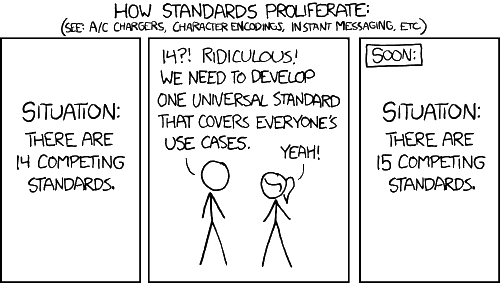
\includegraphics[width=0.7\textwidth]{assets/xkcd_standards_trans.png}
      \label{fig:xkcd_standards}
    \end{center}
    \blankfootnote{\url{https://xkcd.com/927/}}
\end{frame}

\note{
    \begin{outline}
        \1 Also: Keine Standards selber setzen wenn es bereits Standards gibt!
        \1 Diese ""Standards"" finden wir als Design-Patterns
    \1 Um uns eine \textbf{Meinung über Designpattern} (Standardlösungen) zu bilden müssen wir uns \textbf{Paradigmen} (Programmierstile ansehen)
    \end{outline}
}

